\documentclass{article}
\usepackage[UTF8]{ctex}
\usepackage[T1]{fontenc}
\usepackage[utf8]{inputenc}
\usepackage{titlesec}
\usepackage[colorlinks, linkcolor = black]{hyperref}
\usepackage{float}
\usepackage{xcolor}
\usepackage{amsmath}
\usepackage{amssymb}
\usepackage{latexsym}
\usepackage{amsthm}
\usepackage{graphicx}
\usepackage{subcaption}
\usepackage{diagbox}
\renewcommand*\thesubfigure{\roman{subfigure}}

% 增加矩阵两侧括号内侧的空白,新建附参数arraystretch的matrix命令族
\makeatletter
\renewenvironment{pmatrix}
{\left(\mkern10.0mu\env@matrix}
{\endmatrix\mkern10.0mu\right)}
\renewcommand*\env@matrix[1][\arraystretch]{%
	\edef\arraystretch{#1}%
	\hskip -\arraycolsep
	\let\@ifnextchar\new@ifnextchar
	\array{*\c@MaxMatrixCols c}}
\makeatother

\newlength{\depthofsumsign}
\setlength{\depthofsumsign}{\depthof{$\sum$}}
\newcommand{\nsum}[1][1.4]{% only for \displaystyle
    \mathop{%
        \raisebox
            {-#1\depthofsumsign+1\depthofsumsign}
            {\scalebox
                {#1}
                {$\displaystyle\sum$}%
            }
    }
}

\titleformat{\section}[block]{\LARGE\scshape}{\arabic{section}}{1em}{}[]

\title{Homework 7}
\author{PB17000297 罗晏宸}
\date{April 19 2020}

\begin{document}
\maketitle

\section{Exercise 14.12}
两个来自世界上不同地方的宇航员同时用他们自己的望远镜观测了太空中某个小区域内恒星的数目$N$。他们的测量结果分别为$M_1$和$M_2$。通常,测量中会有不超过 1 颗恒星的误差,发生错误的概率$e$很小。每台望远镜可能出现(出现的概率$f$更小一些)对焦不准确的情况(分别记作$F_1$和$F_2$),在这种情况下科学家会少数三颗甚至更多的恒星(或者说,当$N$小于 3 时,连一颗恒星都观测不到)。考虑图\ref{14.22}所示的三种贝叶斯网络结构。
\begin{figure}
    \centering
    \begin{subfigure}[t]{0.3\textwidth}
        \centering
        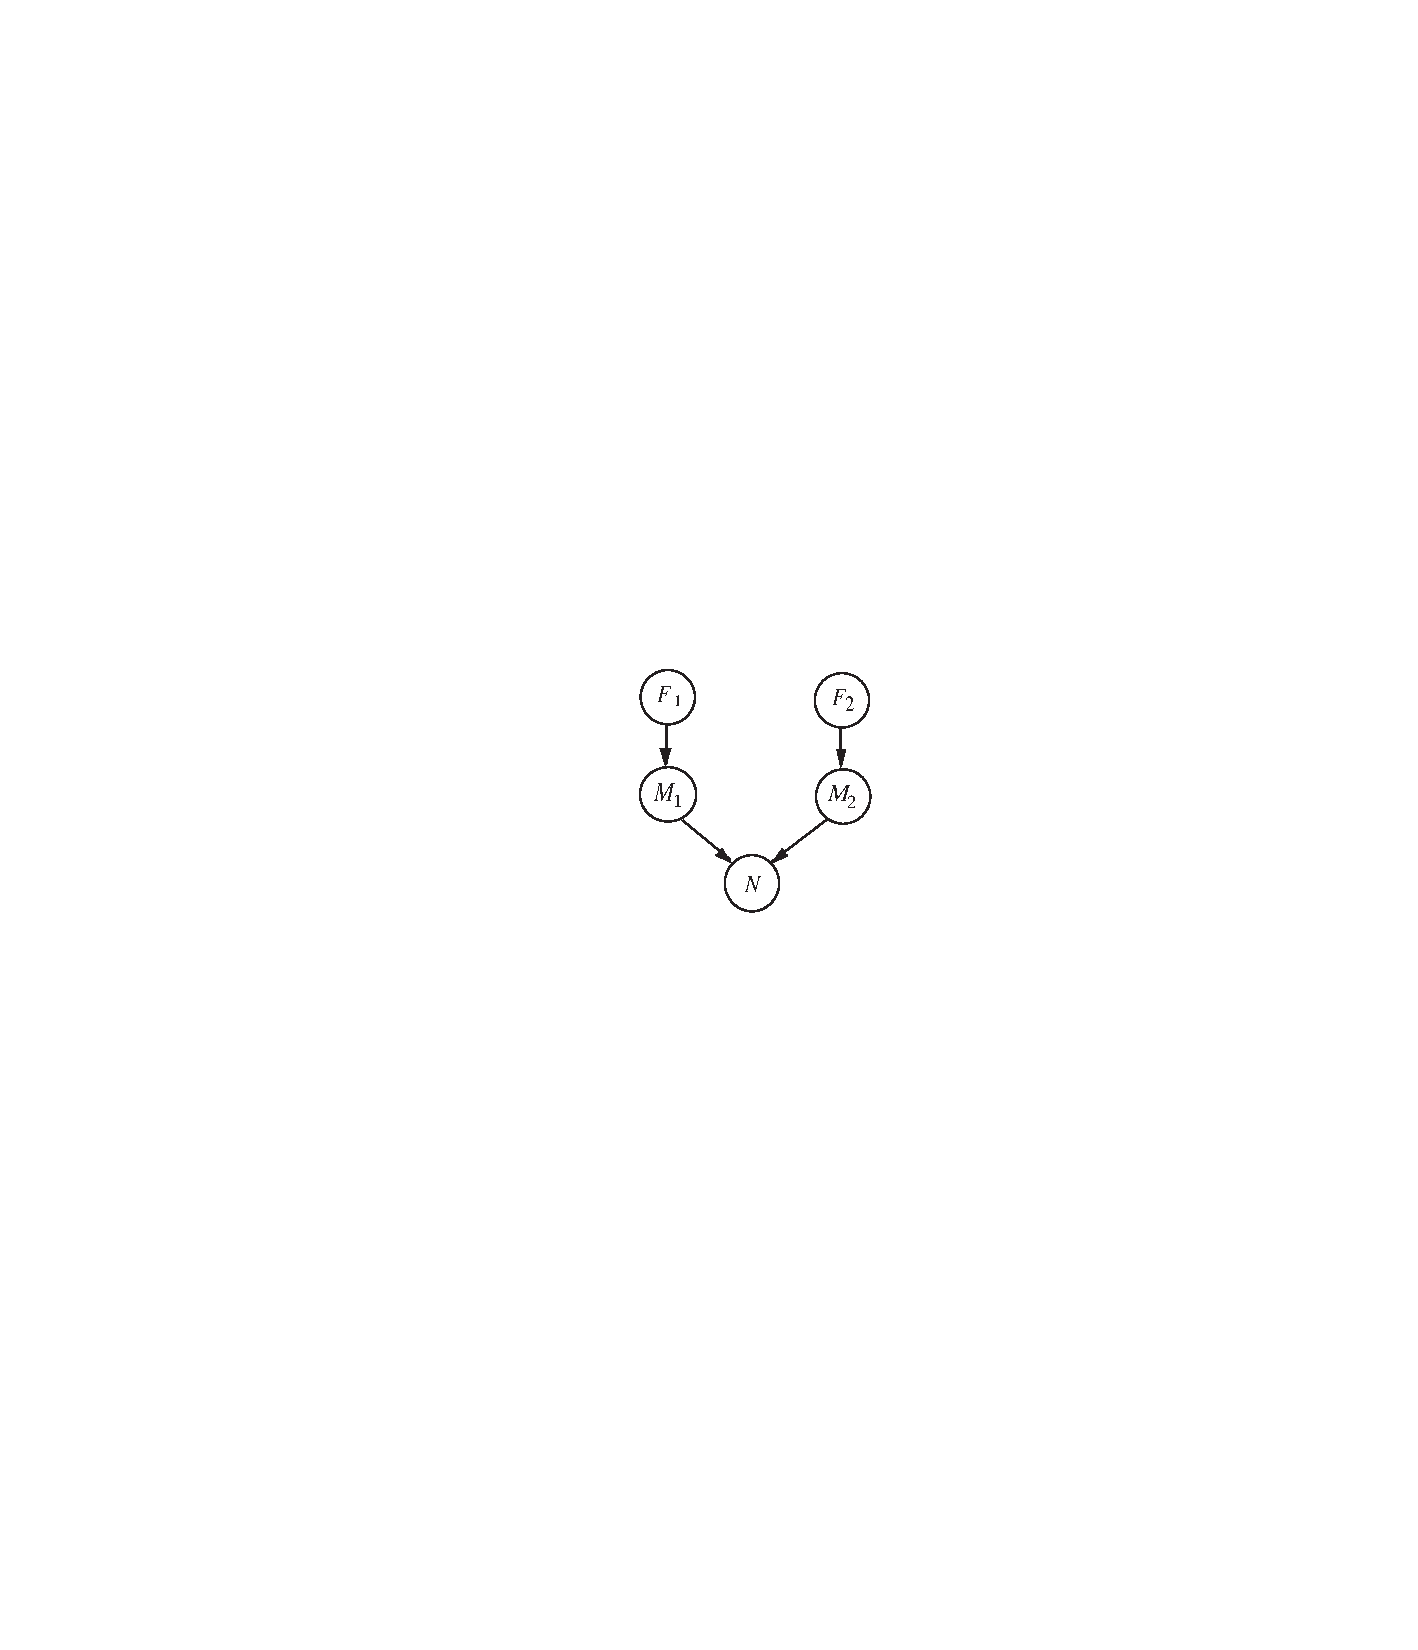
\includegraphics[scale = 0.7]{Figure/14-22(i).pdf}
        \caption{}
        \label{14.22(i)}
    \end{subfigure}
    \begin{subfigure}[t]{0.3\textwidth}
        \centering
        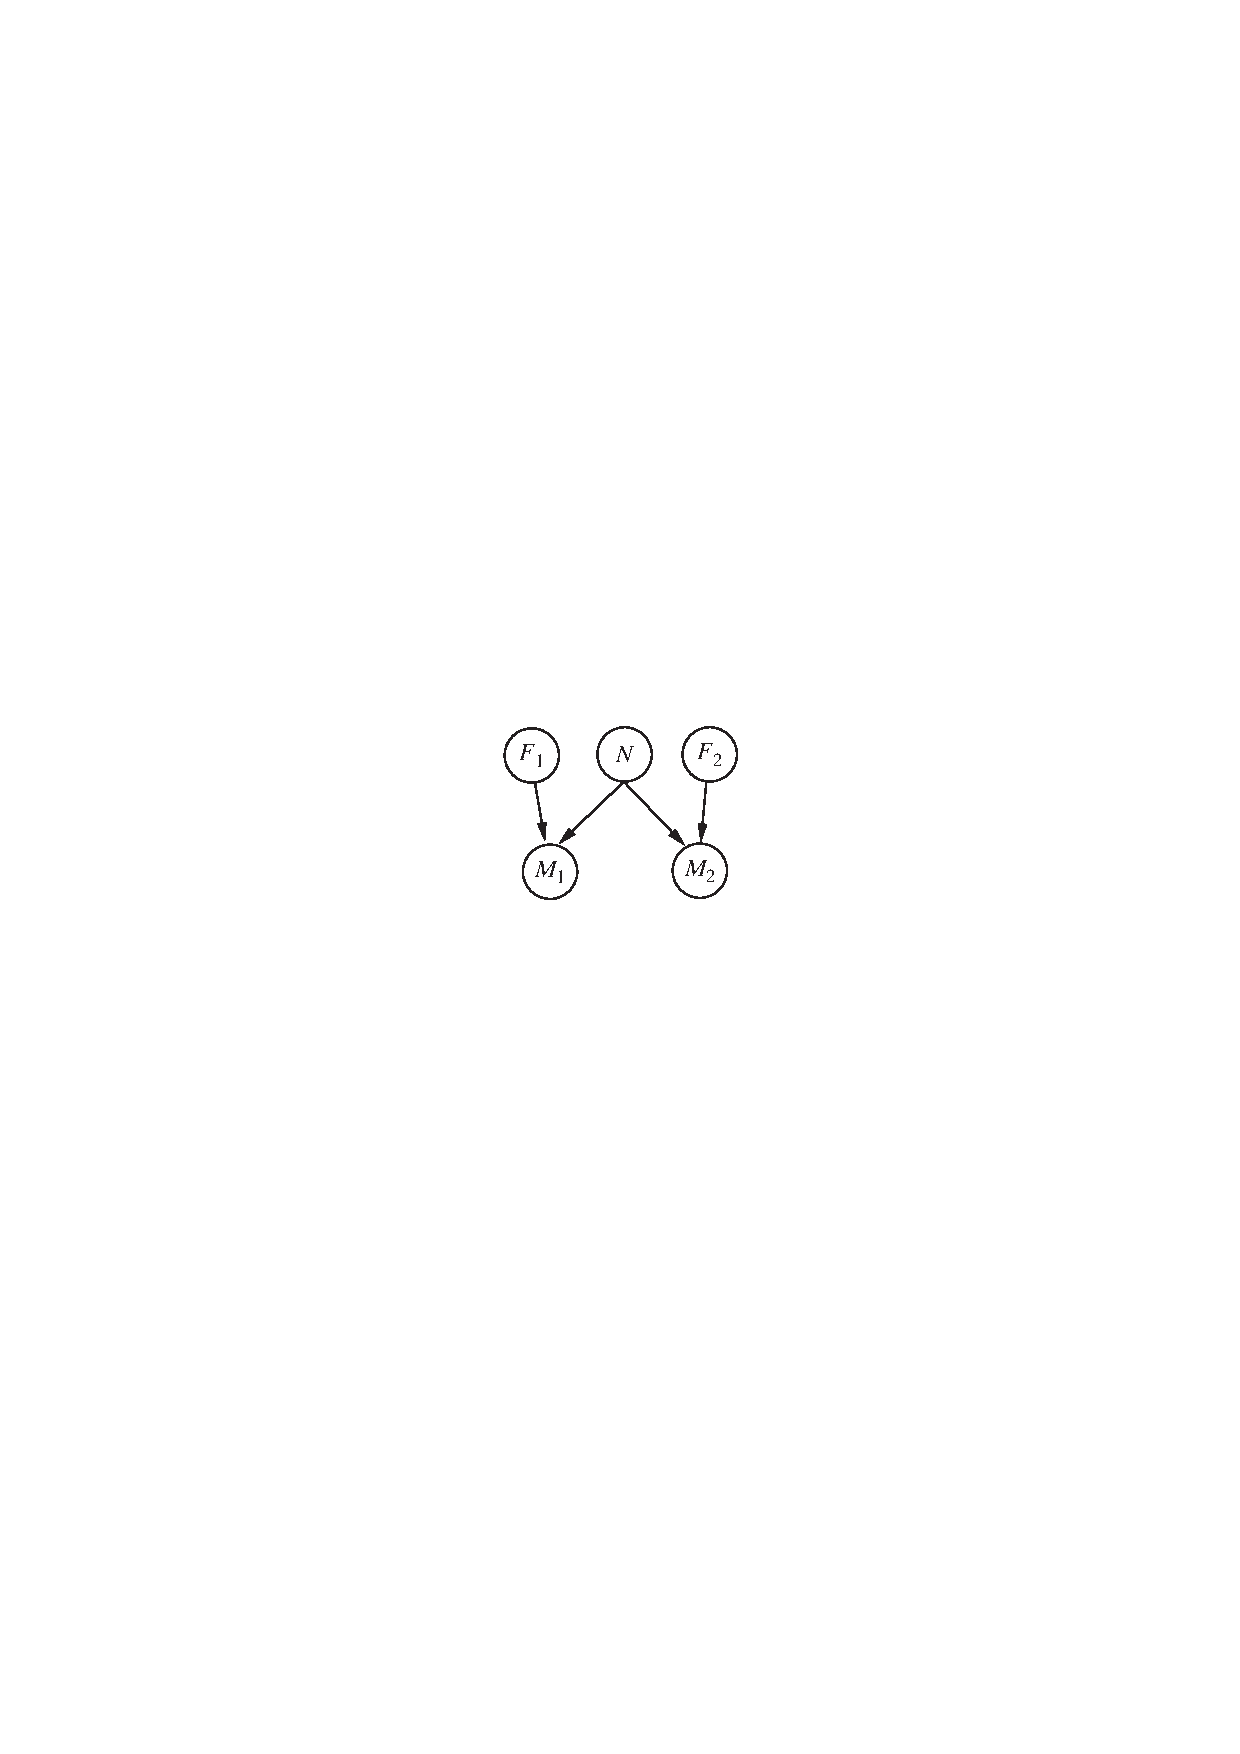
\includegraphics[scale = 0.7]{Figure/14-22(ii).pdf}
        \caption{}
        \label{14.22(ii)}
    \end{subfigure}
    \begin{subfigure}[t]{0.3\textwidth}
        \centering
        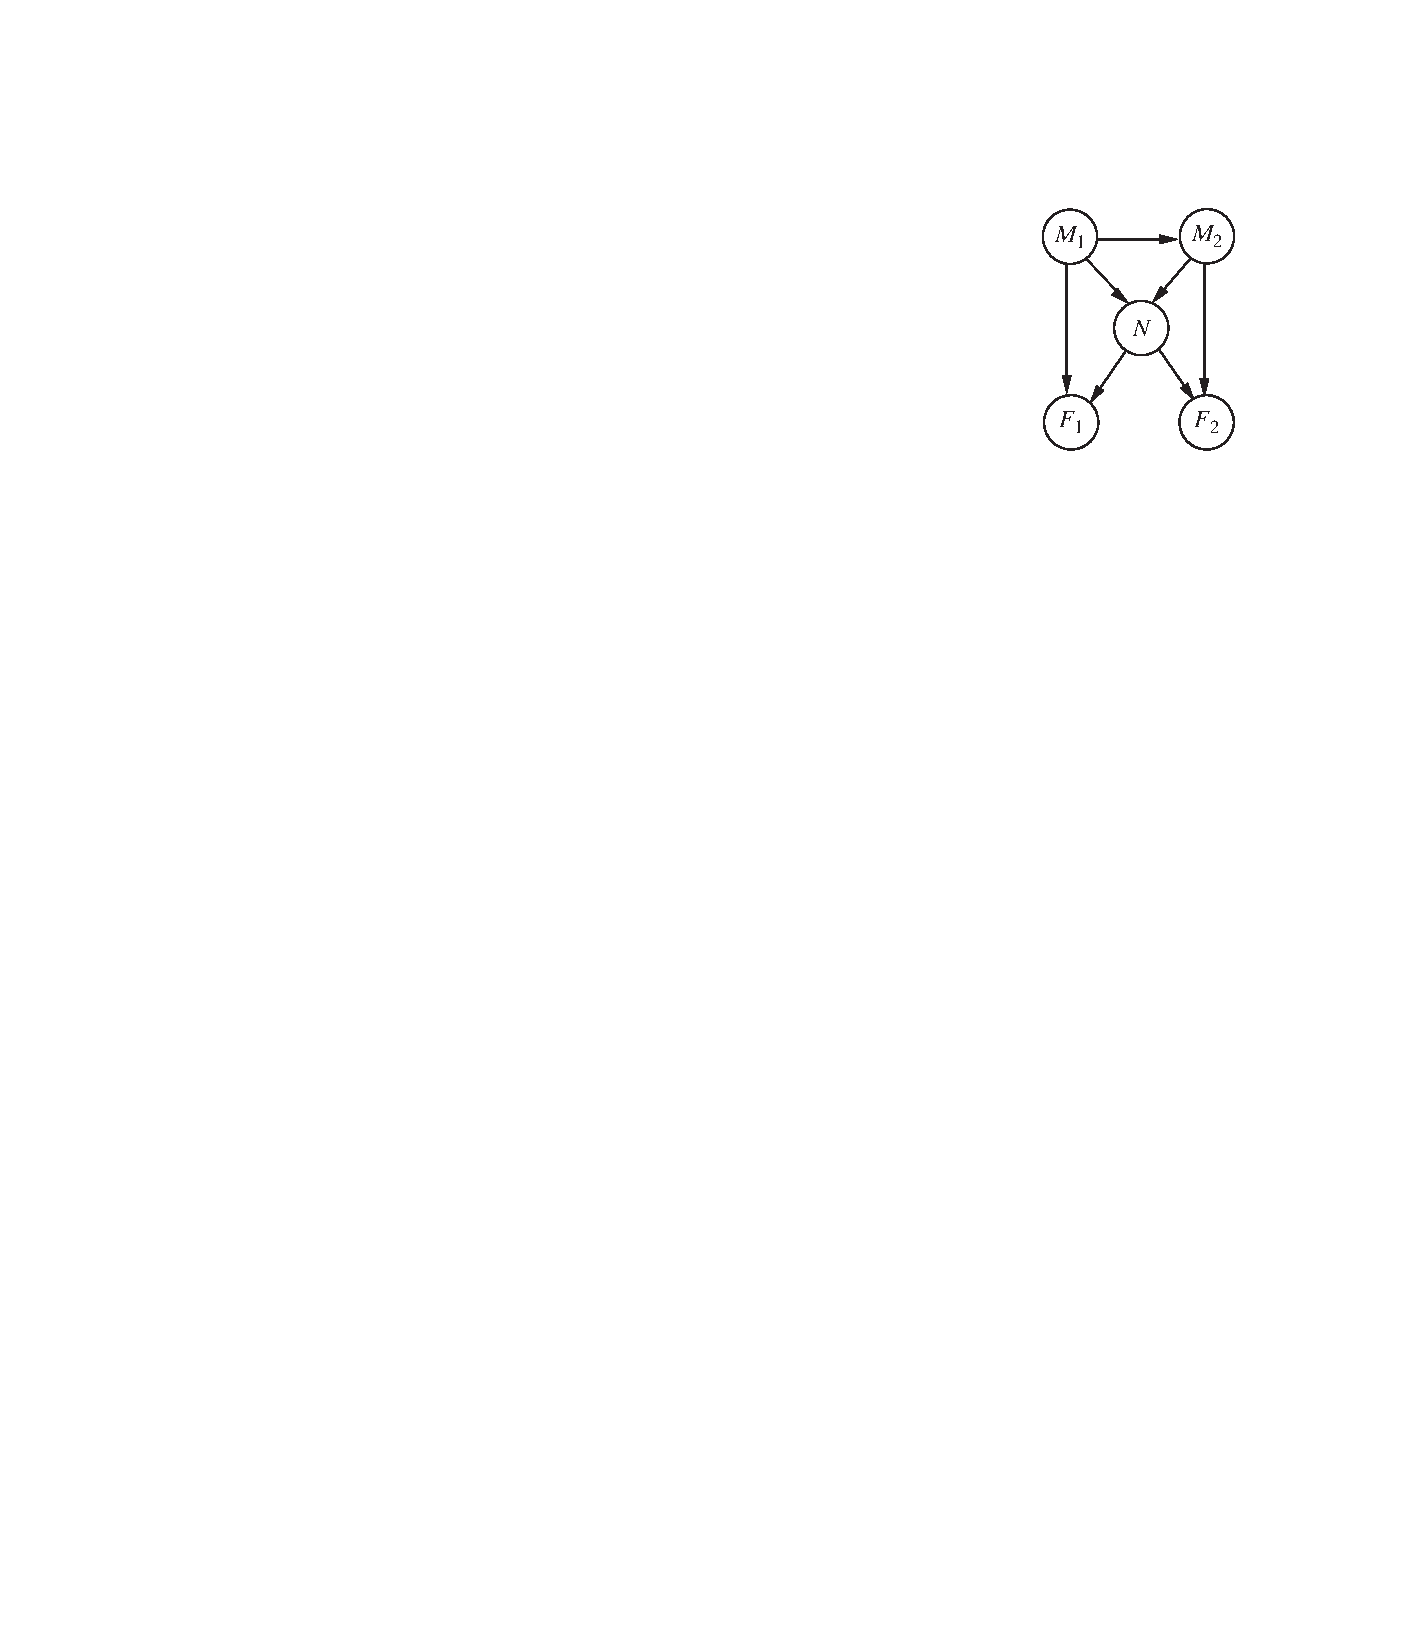
\includegraphics[scale = 0.7]{Figure/14-22(iii).pdf}
        \caption{}
        \label{14.22(iii)}
    \end{subfigure}
    \caption{望远镜问题的三种可能网络}
    \label{14.22}
\end{figure}
\subparagraph{a.} 这三种网络结构哪些是对上述信息的正确(但不一定高效)表示?
\subparagraph{b.} 哪一种网络结构是最好的?请解释。
\subparagraph{c.} 当$N \in \{1,\, 2,\, 3\}$,$M_1 \in \{0,\, 1,\, 2,\, 3,\, 4\}$时,请写出$\mathbf{P}(M_1 | N)$的条件概率表。概率分布表里的每个条目都应该表达为参数$e$和/或$f$的一个函数。

\paragraph{解}
\subparagraph{a.}
网络(\subref{14.22(ii)})和(\subref{14.22(iii)})都是正确的表示。虽然(\subref{14.22(i)})描述了计算过程,但没有准确描述恒星数目$N$和对焦情况的关系,因此不是一个贝叶斯网络结构;(\subref{14.22(ii)})对因果结构的表示是正确的,两台望远镜的对焦情况彼此独立,测量结果受实际恒星数量和对焦情况的影响;(\subref{14.22(iii)})也是正确的,其是对结点排序之后的结果。

\subparagraph{b.}
(\subref{14.22(ii)})比(\subref{14.22(iii)})需要更少的参数,因此网络(\subref{14.22(ii)})是最好的。

\subparagraph{c.} 对概率展开有
\begin{align*}
    \mathbf{P}(M_1 | N) & = \mathbf{P}(M_1 | N,\, F_1)\mathbf{P}(F_1 | N) + \mathbf{P}(M_1 | N,\, \lnot F_1)\mathbf{P}(\lnot F_1 | N) \\
                        & = \mathbf{P}(M_1 | N,\, F_1)\mathbf{P}(F_1) + \mathbf{P}(M_1 | N,\, \lnot F_1)\mathbf{P}(\lnot F_1)         \\
                        & = \mathbf{P}(M_1 | N,\, F_1)f + \mathbf{P}(M_1 | N,\, \lnot F_1)(1 - f)
\end{align*}
假设测量时发生的多数1颗恒星和少数1颗恒星的概率均为$\dfrac{e}{2}$计算得到条件概率表如下:
\begin{table}[h]
    \centering
    \begin{tabular}{|c|c|c|c|}
        \hline
        \diagbox{$M_1$}{$\mathbf{P}(M_1 | N)$}{N} & $1$                      & $2$                  & $3$                  \\
        \hline $0$                                & $f + \frac{e}{2}(1 - f)$ & $f$                  & $f$                  \\
        \hline $1$                                & $(1 - e)(1 - f)$         & $\frac{e}{2}(1 - f)$ & $0$                  \\
        \hline $2$                                & $\frac{e}{2}(1 - f)$     & $(1 - e)(1 - f)$     & $\frac{e}{2}(1 - f)$ \\
        \hline $3$                                & $0$                      & $\frac{e}{2}(1 - f)$ & $(1 - e)(1 - f)$     \\
        \hline $4$                                & $0$                      & $0$                  & $\frac{e}{2}(1 - f)$ \\
        \hline
    \end{tabular}
    \caption{当$N \in \{1,\, 2,\, 3\}$,$M_1 \in \{0,\, 1,\, 2,\, 3,\, 4\}$时$\mathbf{P}(M_1 | N)$的条件概率表}
    \label{table}
\end{table}

\section{Exercise 14.13}
考虑图\ref{14.22}(\subref{14.22(ii)})的网络,假设两个望远镜完全相同。$N \in \{1,\, 2,\, 3\}$,$M_1,\, M_2 \in \{0,\, 1,\, 2,\, 3,\, 4\}$,CPT 表和习题14.12所描述的一样。使用枚举算法(图\ref{14.9})计算概率分布$\mathbf{P}(N | M_1 = 2,\, M_2 = 2)$。
\begin{figure}
    \centering
    \fbox{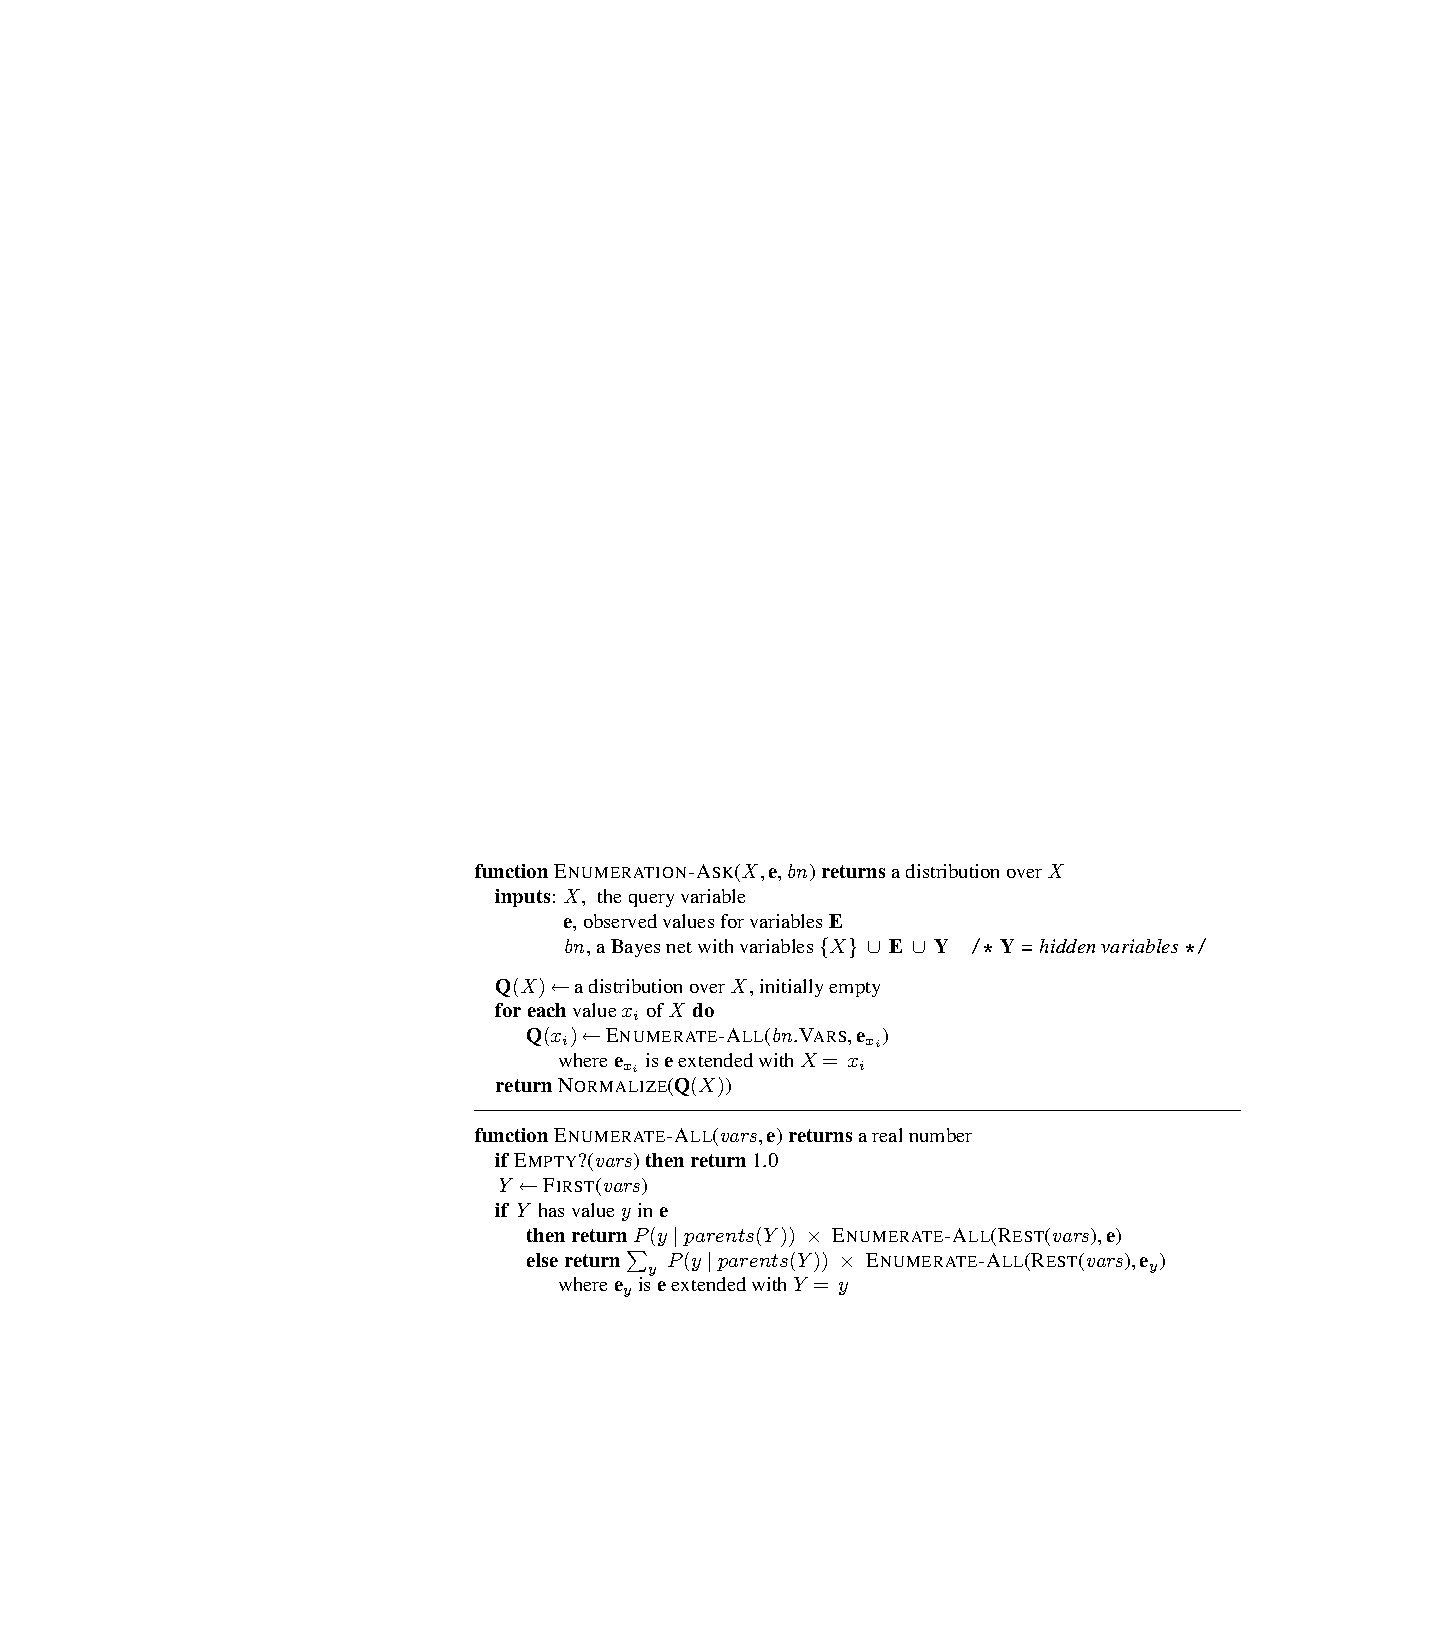
\includegraphics[width = \textwidth]{Figure/14-9.pdf}}
    \caption{在贝叶斯网络上回答查询的枚举算法}
    \label{14.9}
\end{figure}

\paragraph{解}
使用枚举算法计算的概率分布如下
\begin{align*}
        & \mathbf{P}(N | M_1 = 2,\, M_2 = 2)                                                                                                                                            \\
    =\  & \alpha \sum_{f_1, f_2}\mathbf{P}(f_1,\, f_2,\, N,\, M_1 = 2,\, M_2 = 2)                                                                                                       \\
    =\  & \alpha \sum_{f_1,f_2}\mathbf{P}(f_1)\mathbf{P}(f_2)\mathbf{P}(M_1 = 2 | f_1,\, N)\mathbf{P}(M_2 = 2 | f_2,\, N)                                                               \\
    =\  & \alpha(1 - f)(1 - f)\left\langle p_1, p_2, p_3\right\rangle\left\langle \frac{e}{2}, 1 - e, \frac{e}{2}\right\rangle\left\langle \frac{e}{2}, 1 - e, \frac{e}{2}\right\rangle \\
    =\  & \alpha'\left\langle p_1\frac{e^2}{4}, p_2(1 - e)^2, p_3\frac{e^2}{4}\right\rangle
\end{align*}

\section{Exercise 14.15}
考虑图\ref{14.11}中的变量消元算法。
\begin{figure}
    \centering
    \fbox{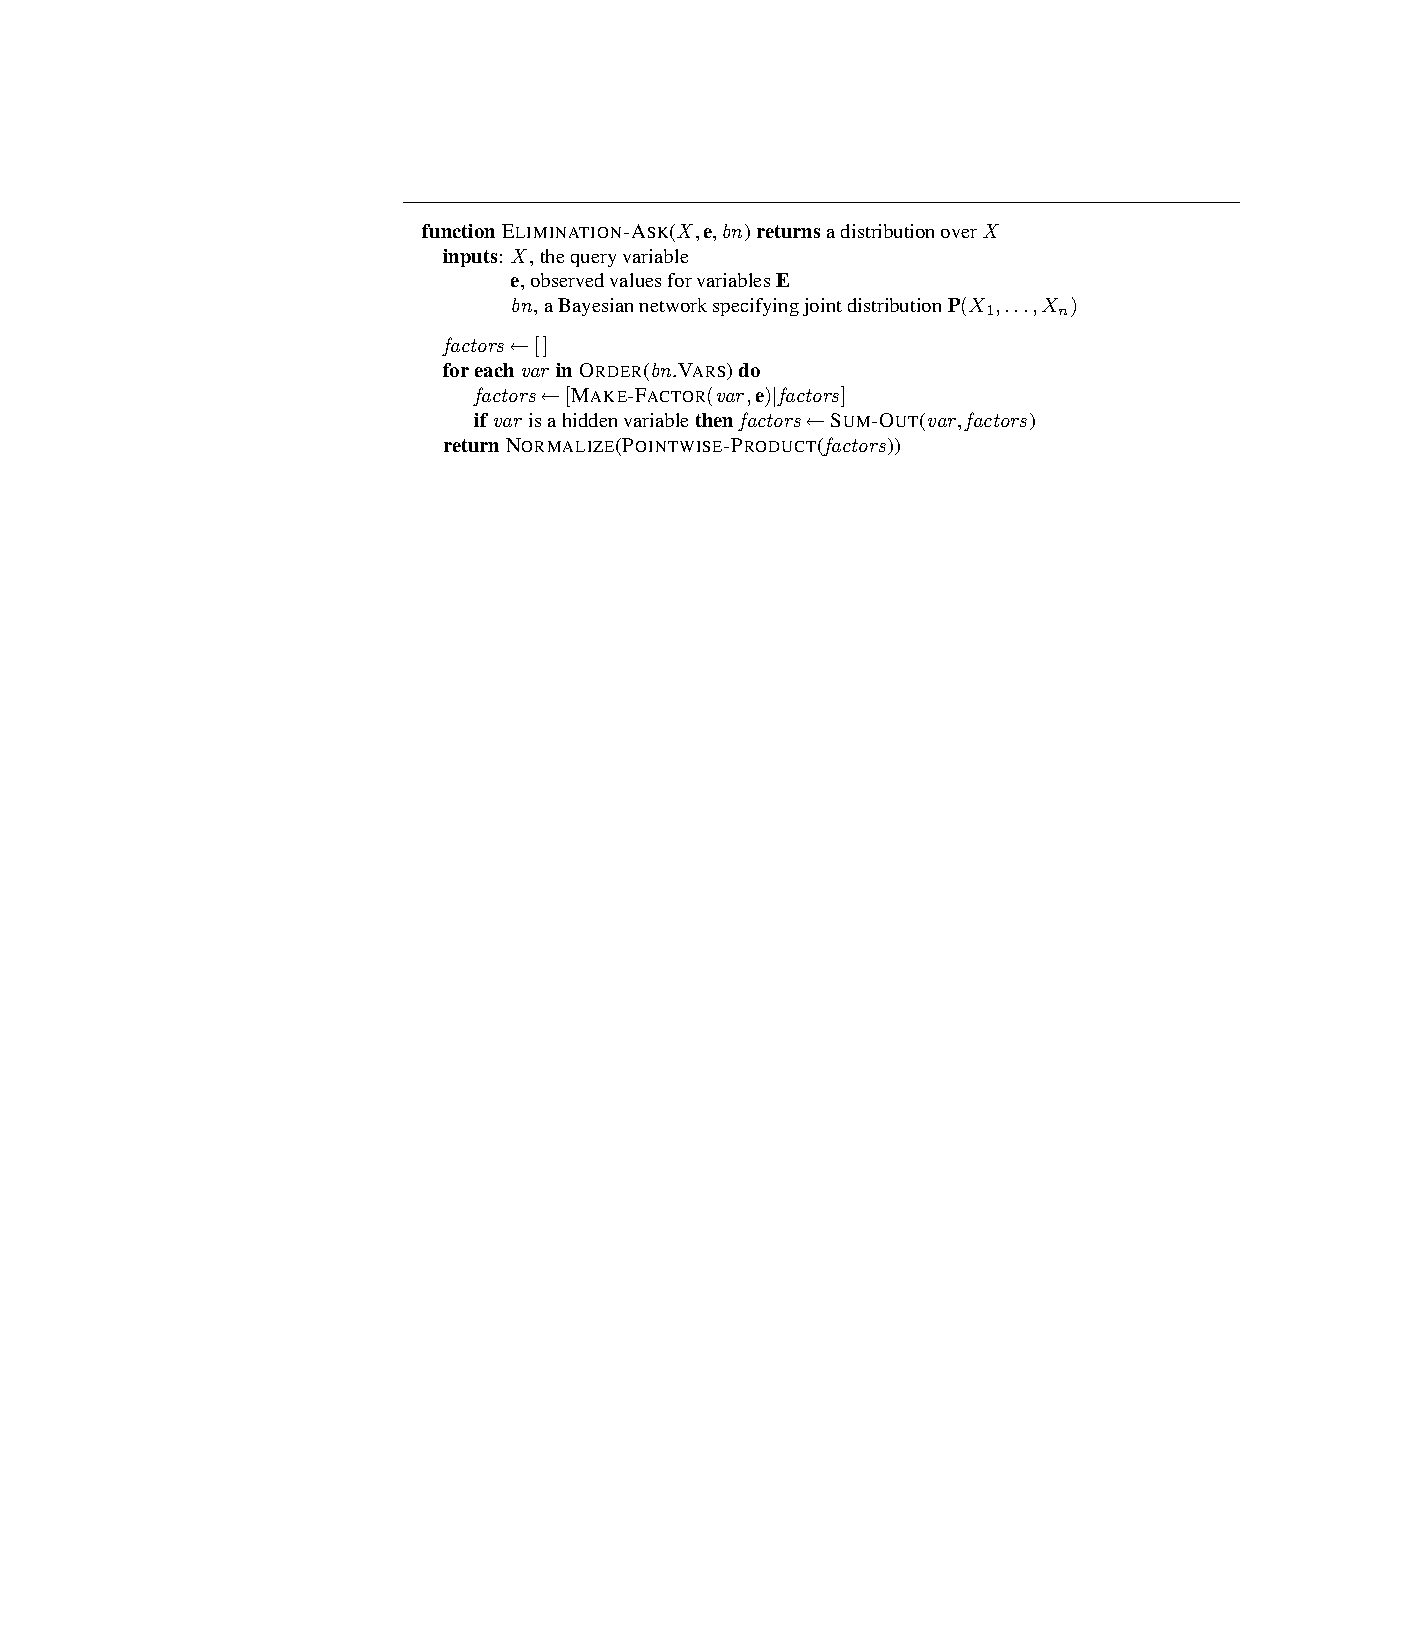
\includegraphics[width = \textwidth]{Figure/14-11.pdf}}
    \caption{用于贝叶斯网络推理的变量消元算法}
    \label{14.11}
\end{figure}
\subparagraph{a} 14.4节对如下查询应用了变量消元算法$$\mathbf{P}(\textit{Burglary}\ |\ \textit{JohnCalls} = \textit{true},\, \textit{MaryCalls} = \textit{true})$$执行必要的计算,并检验计算结果的正确性。
\subparagraph{b} 统计所执行的算术运算的次数,将其与枚举算法所需的运算次数进行比较。
\subparagraph{c} 假设贝叶斯网络结构具有链式结构,即由一个布尔随机变量序列$X_1,\, \cdots,\, X_n$构成,其中$\textit{Parents}(X_i) = \{X_{i - 1}\},\ i = 2,\, \cdots,\, n$。请问使用枚举算法计算$\mathbf{P}(X_1 | X_n = \textit{true})$的复杂度是多少?使用变量消元算法呢?

\paragraph{解}
\subparagraph{a} 计算表达式
\begin{align*}
              & \mathbf{P}(\textit{Burglary}\ |\ \textit{JohnCalls} = \textit{true},\, \textit{MaryCalls} = \textit{true})    \\
    =\        & \mathbf{P}(b | j,\, m)                                                                                        \\
    =\        & \alpha \mathbf{P}(b) \sum_{e} P(e)\sum_{a} \mathbf{P}(a | b,\, e)P(j | a)P(m | a)                             \\
    =\        & \alpha \mathbf{P}(b) \nsum[3.2]_{e}P(e)\left[
        \begin{pmatrix}[1.5]
            P(a | b,\, e)       & P(a | \lnot b,\, e)       \\
            P(a | b,\, \lnot e) & P(a | \lnot b,\, \lnot e)
        \end{pmatrix}
        P(j | a)P(m | a)                                                                                              \right. \\
              & \indent +
        \left.
        \begin{pmatrix}[1.5]
            P(\lnot a | b,\, e)       & P(\lnot a | \lnot b,\, e)       \\
            P(\lnot a | b,\, \lnot e) & P(\lnot a | \lnot b,\, \lnot e)
        \end{pmatrix}
        P(j | \lnot a)P(m | \lnot a)\right]                                                                                   \\
    =\        & \alpha \mathbf{P}(b)  \nsum[2.0]_{e}P(e)\left[
        \begin{pmatrix}
            0.95 & 0.29  \\
            0.94 & 0.001
        \end{pmatrix}
        \times 0.90 \times 0.70  \right.                                                                                      \\
              & \indent +
        \left.
        \begin{pmatrix}
            0.05 & 0.71  \\
            0.06 & 0.999
        \end{pmatrix}
        \times 0.05 \times 0.01\right]                                                                                        \\
    =\        & \alpha \mathbf{P}(b)  \nsum[2.0]_{e}P(e)
    \begin{pmatrix}
        0.598525 & 0.183055  \\
        0.59223  & 0.0011295 \\
    \end{pmatrix}                                                                                                \\
    =\        & \alpha \mathbf{P}(b) \left[
        \begin{pmatrix}
            0.598525 \\
            0.183055
        \end{pmatrix}  \times 0.002 +
        \begin{pmatrix}
            0.59223 \\
            0.0011295
        \end{pmatrix}  \times 0.998   \right]                                                                    \\
    =\        & \alpha \mathbf{P}(b)
    \begin{pmatrix}
        0.59224259  \\
        0.001493351 \\
    \end{pmatrix}                                                                                                \\
    =\        & \alpha \langle 0.001 \times 0.59224259, 0.999 \times 0.001493351 \rangle                                      \\
    =\        & \alpha \langle 0.00059224259, 0.001491857649 \rangle                                                          \\
    \approx\  & \langle 0.284, 0.716 \rangle
\end{align*}
结果是正确的

\subparagraph{b}
在上述的算术运算中,共有7次加法,16次乘法和2次除法。枚举算法有7次加法,18次乘法和2次除法,相比之下需要2次额外的乘法。

\subparagraph{c}
使用枚举算法计算$\mathbf{P}(X_1 | X_n = \textit{true})$,对于随机变量$X_1$的两种取值,分别需要计算两棵深度均为$n - 2$的二叉树,因此复杂度是$O(2^n)$的。

使用变量消元算法计算$\mathbf{P}(X_1 | X_n = \textit{true})$,可以归纳地得到规模$n - 1,\, n - 2,\, \cdots,\, 1$的子问题,且递推是常数时间的,因此总的复杂度是$O(n)$的。
\end{document}